\section{Locality}
In a modern computer, memory is arranged in a subsequent manner,
different types of memory are used in order to keep cost down and
speed up. Closer to the CPU small and fast memory types are used those
are often referred to as cache memories and are an intermediate memory
level between the CPU registers and the RAM. In today's computers,
usually several layers of cache memories are used. A schematic image
of this is shown in fig. \ref{fig:hpc:mem}.

\begin{figure}
\begin{center}
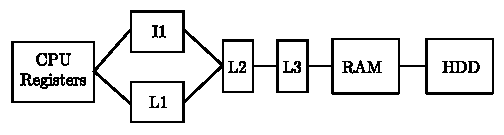
\includegraphics[width=0.6\textwidth]{fig/mem.pdf}
\end{center}
\caption{Sketch of memory layout in a modern computer. I1 is the
  instruction cache and L1 the smallest data cache. Memories to the
  left are faster and smaller but more expensive. }
\label{fig:hpc:mem}
\end{figure}

When data are to be fetched from the memory into the registers of the
CPU, it is first looked for in the L1 data cache if it is not present
there, the next level cache (L2) are tried and so on. If the data is
not present in any level of the cache it has to be read from the main
memory, this is often referred to as a cache miss and is the opposite
to a cache hit. To fetch data from the main memory takes, for a modern
CPU, the same amount of time in which the CPU may execute about 100
instructions \cite{wiki-mem}. It is in other words much slower than to
fetch from the cache.

As a cache miss occurs, not only the value at the specific address
that was wanted but also data that is adjacent to that value is
fetched and placed in the cache. This collection of data is called a
cache line. In order to keep down memory latency, it may be a good
idea if the other data in the cache line could be used before it is
overwritten. This is the concept of locality, to keep data adjacent in
memory that are to be used adjacent in time. It is a major topic in
high performance computing and great performance losses may arise if
the principle of locality is not considered.

%\todo{example}

\subsection{Locality and the LBM}
In an implementation of the lattice-Boltzmann method, the main
quantity that is used in computation is the distribution
function $\fii$. It is in the implementation realised as an array of
dimension $\nx \times \ny \times Q$ where $Q$ is the number of
directions in the discretised velocity space. Basically, two models
for arranging $\fii$ in memory exist:

\begin{description}
  \item[A.] All directions for a certain node are placed adjacent in
    memory.
  \item[B.] All nodes for a certain direction are placed adjacent in
    memory.
\end{description}

To decide which model that is chosen, they must be examined with
respect to locality and the algorithm used. The algorithm in the LBM
consists of two main parts, i.e. the collision step and the streaming
step. In a BGK collision, to update $\fii$, i.e. the distribution
function for direction $i$, the distribution functions for all other
directions from this node must be used in order to compute the
equilibrium distribution. Thus for the collision step, model A would
give better locality. On the other hand, in the streaming step, to
stream $\fii$, the streaming must start at the nodes where, $i$ is
directed out of the domain. Otherwise will unstreamed distributions be
overwritten. Thus it is not directly possible to stream all directions
for a certain node adjacent in time but instead all nodes for a
certain direction. This suggests that model B is more favourable for
the streaming step. There is an approach proposed in \cite{mikael}
where two arrays are used for $\fii$ and in the streaming step, the
streaming is done from one array to the other and nothing is
overwritten. This requires however twice as much memory and it has not
been tested in the implementation done in this work.

$Q$ is typically much smaller than the number of nodes $\nx \times
\ny$. This gives that when a cache line is fetched for model A, same
directions from neighbouring nodes will also be fetched into the cache
and a cache miss will not occur for each node update in the
streaming. In model B, different directions will typically not be
fetched for the same node and in the collision step, a cache miss will
probably occur for each direction. The conclusion is that model A is
better with respect to locality for the ``worst'' part of the
algorithm and is therefore chosen. Tests performed on a laptop with
an Intel Core 2 Duo processor also shows that model A in general gives
better locality.


\nomenclature{L1, L2, L3}{Level 1,2,3 (cache)}
\nomenclature{RAM}{Random Access Memory}
\nomenclature{HDD}{Hard Disk Drive}
